
\begin{frame}
  \frametitle{Prediction Using Nuclide Masses}
  \begin{figure}
    \centering
    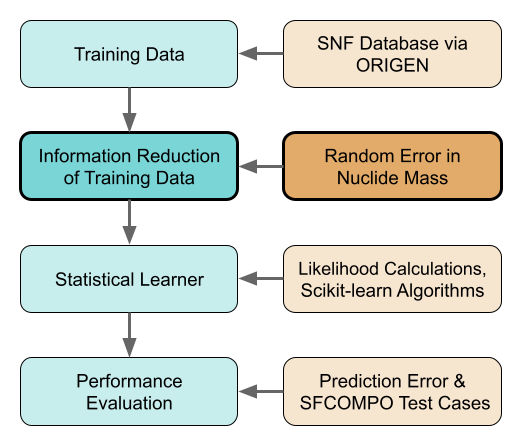
\includegraphics[width=0.6\textwidth]{./figures/methodology1_pres.png}
  \end{figure}
\end{frame}

\begin{frame}
  \frametitle{Information Reduction: Random \& Uniform Error}
  \begin{block}{Scikit-learn Algorithms}
    \small
    Introduced $0\% < E_{max} < 20\%$ random error:
    \[E_{max} = \text{0, 1, 2, 5, 8, 10, 12, 15, 18, 20}\% \]
    Each nuclide measurement is altered by a random percentage in the range: 
    \[[100-E_{max},100+E_{max}]\]
  \end{block}
  \begin{block}{Maximum Likelihood Calculations}
  \small
    Introduced uniform simulation uncertainty: 
    \[\sigma_i = \text{1, 5, 10, 15, 20}\% \]
    Each nuclide measurement is given a standard deviation via 
    \cite{mll_sensitivity}:
    \[\sigma_{Log L}^2 = \sum_i \left( 
                                \frac{x_{i,test} - x_{i,train}}{\sigma_{i,train}^2}
                                \right)^2 
                                (\sigma_{i,train}^2 + \sigma_{i,test}^2)
    \]
  \end{block}
\end{frame}

\begin{frame}
  \frametitle{Reactor Type Classification}
    \begin{figure}
      \centering
      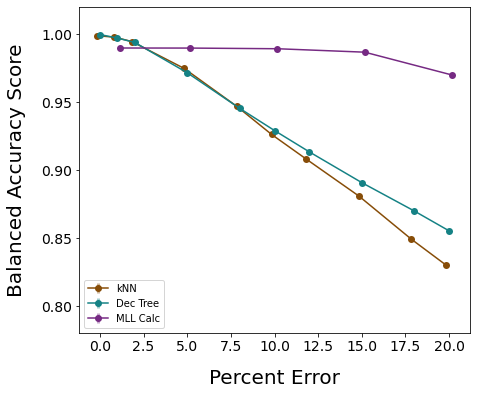
\includegraphics[width=0.6\textwidth]{./figures/randerr_compare_nuc29_BalAcc_rxtr.png}
      \\ \scriptsize (99.9\% confidence interval error bars)
    \end{figure}
\end{frame}

\begin{frame}
  \frametitle{Reactor Type Classification}
    \begin{figure}
      \centering
      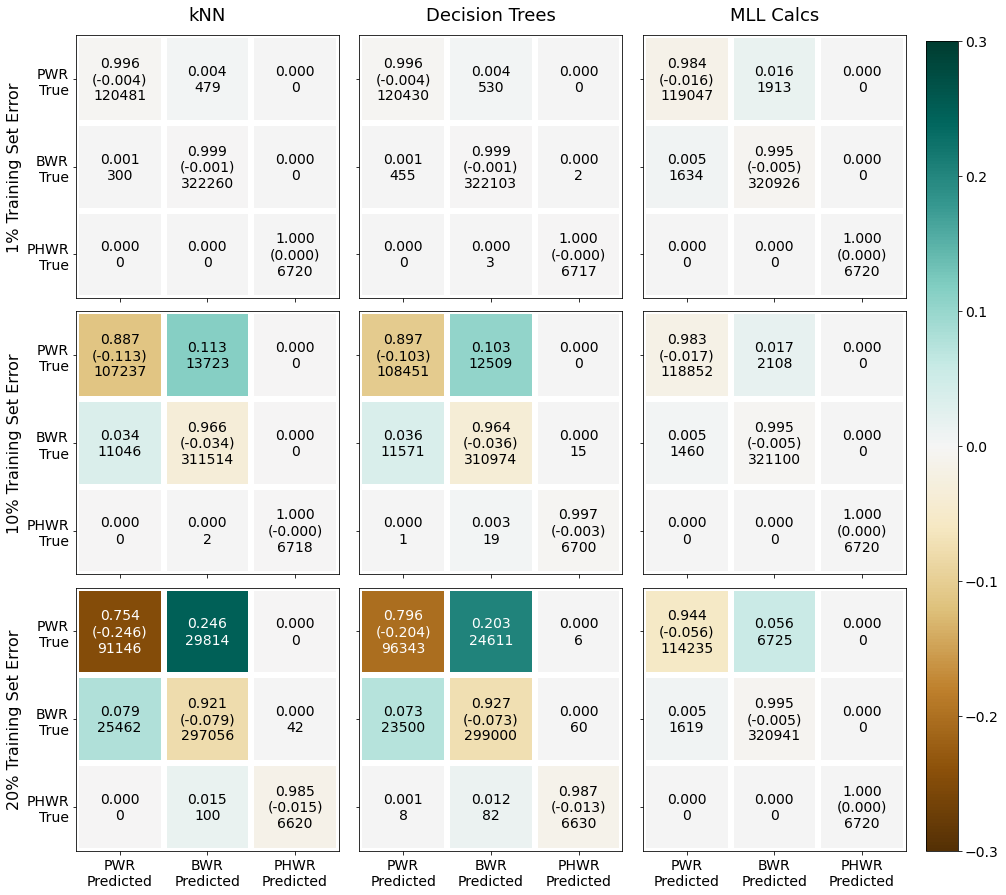
\includegraphics[height=0.85\textheight]{./figures/confusion_matrix_nuc29_3errs.png}
    \end{figure}
\end{frame}

\begin{frame}
  \frametitle{Burnup Regression}
  \begin{adjustwidth}{-15pt}{-5pt}
  \begin{minipage}{0.5\textwidth}
    \begin{figure}
      \centering
      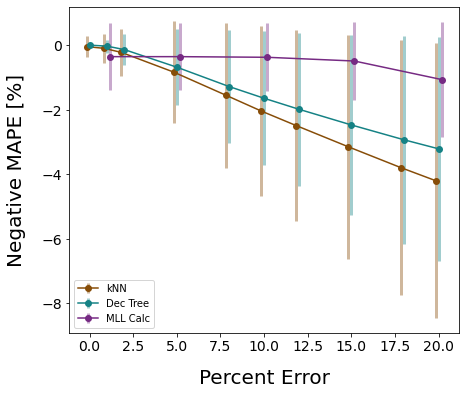
\includegraphics[width=\textwidth]{./figures/randerr_compare_nuc29_MAPE_burn.png}
      \scriptsize (1-sigma error bars)
    \end{figure}
  \end{minipage}%
  \hfill
  \begin{minipage}{0.5\textwidth}
    \begin{figure}
      \centering
      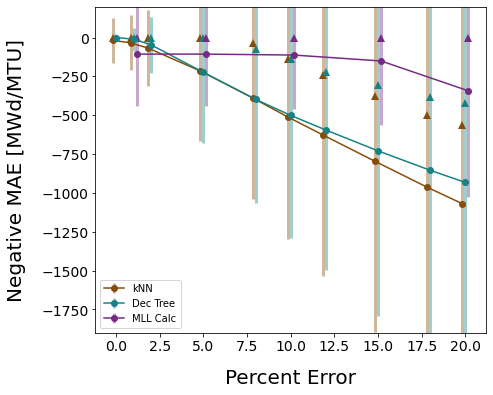
\includegraphics[width=1.05\textwidth]{./figures/randerr_compare_nuc29_MAE_burn.png}
      \scriptsize (1-sigma error bars)
    \end{figure}
  \end{minipage}
  \end{adjustwidth}
\end{frame}

\begin{frame}
  \frametitle{${}^{235}\text{U}$ Enrichment Regression}
  \begin{adjustwidth}{-15pt}{-5pt}
  \begin{minipage}{0.5\textwidth}
    \begin{figure}
      \centering
      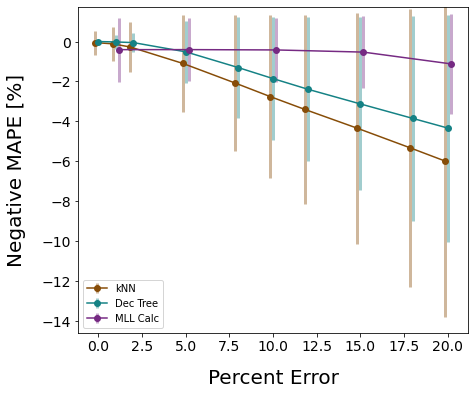
\includegraphics[width=\textwidth]{./figures/randerr_compare_nuc29_MAPE_enri.png}
      \scriptsize (1-sigma error bars)
    \end{figure}
  \end{minipage}%
  \hfill
  \begin{minipage}{0.5\textwidth}
    \begin{figure}
      \centering
      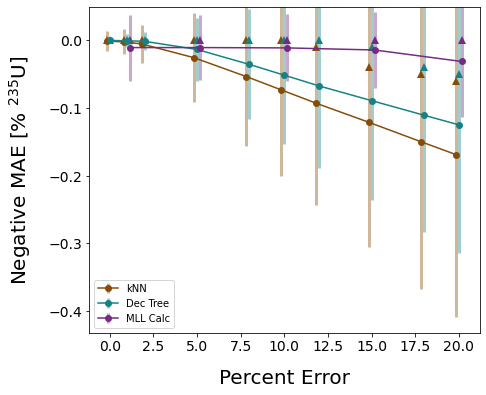
\includegraphics[width=1.05\textwidth]{./figures/randerr_compare_nuc29_MAE_enri.png}
      \scriptsize (1-sigma error bars)
    \end{figure}
  \end{minipage}
  \end{adjustwidth}
\end{frame}

\begin{frame}
  \frametitle{Time Since Irradiation Regression}
  \begin{adjustwidth}{-15pt}{-5pt}
  \begin{minipage}{0.5\textwidth}
    \begin{figure}
      \centering
      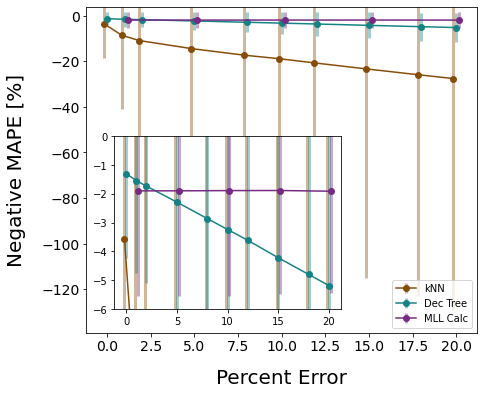
\includegraphics[width=\textwidth]{./figures/randerr_compare_nuc29_MAPE_cool.png}
      \scriptsize (1-sigma error bars)
    \end{figure}
  \end{minipage}%
  \hfill
  \begin{minipage}{0.5\textwidth}
    \begin{figure}
      \centering
      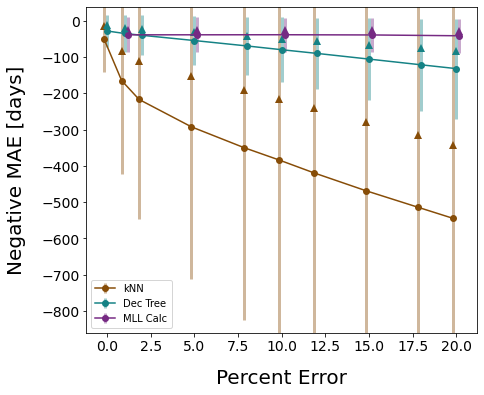
\includegraphics[width=1.05\textwidth]{./figures/randerr_compare_nuc29_MAE_cool.png}
      \scriptsize (1-sigma error bars)
    \end{figure}
  \end{minipage}
  \end{adjustwidth}
\end{frame}

\begin{frame}
  \frametitle{SFCOMPO Database as Test Cases}
  \begin{adjustwidth}{-10pt}{-10pt}
  \vspace{-8pt}
  \begin{minipage}[t]{0.45\textwidth}
    \begin{block}{505 Test Cases}
      Range of reactor operation parameters in SFCOMPO:
      \begin{figure}
        \centering
        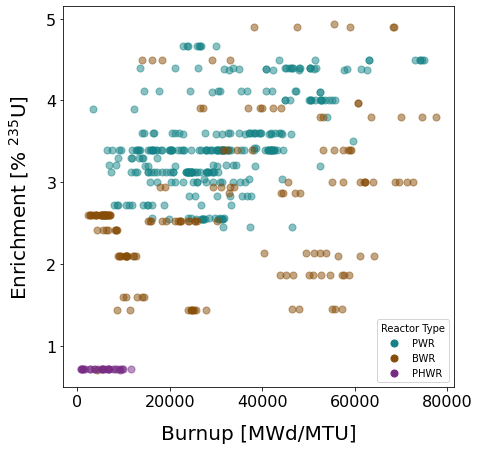
\includegraphics[width=\textwidth]{./figures/sfcompo_scatter_viz.png}
      \end{figure}
    \end{block}
  \end{minipage}%
  \hfill
  \begin{minipage}[t]{0.57\textwidth}
    \begin{block}{Many Missing Features}
      Number of assays each nuclide is measured for in SFCOMPO:
      \begin{table}
        \footnotesize
        \centering
        \renewcommand{\arraystretch}{1.3}
        \begin{tabular}{>{\raggedleft}m{0.32in}
                                      m{0.16in}|
                        >{\raggedleft}m{0.32in}
                                      m{0.16in}|
                        >{\raggedleft}m{0.32in}
                                      m{0.16in}}
          \toprule
          \rowcolor[gray]{0.88} ${}^{241}\text{Am}$  & 237 & ${}^{145}\text{Nd}$ & 162 & ${}^{147}\text{Sm}$ & 97  \\  
          \rowcolor[gray]{0.95} ${}^{242m}\text{Am}$ & 110 & ${}^{146}\text{Nd}$ & 139 & ${}^{149}\text{Sm}$ & 97  \\ 
          \rowcolor[gray]{0.88} ${}^{243}\text{Am}$  & 203 & ${}^{148}\text{Nd}$ & 275 & ${}^{150}\text{Sm}$ & 97  \\ 
          \rowcolor[gray]{0.95} ${}^{242}\text{Cm}$  & 214 & ${}^{150}\text{Nd}$ & 121 & ${}^{151}\text{Sm}$ & 97  \\ 
          \rowcolor[gray]{0.88} ${}^{244}\text{Cm}$  & 269 & ${}^{237}\text{Np}$ & 155 & ${}^{152}\text{Sm}$ & 97  \\ 
          \rowcolor[gray]{0.95} ${}^{134}\text{Cs}$  & 113 & ${}^{238}\text{Pu}$ & 369 & ${}^{234}\text{U}$  & 355 \\ 
          \rowcolor[gray]{0.88} ${}^{137}\text{Cs}$  & 185 & ${}^{239}\text{Pu}$ & 505 & ${}^{235}\text{U}$  & 479 \\ 
          \rowcolor[gray]{0.95} ${}^{154}\text{Eu}$  & 100 & ${}^{240}\text{Pu}$ & 505 & ${}^{236}\text{U}$  & 462 \\ 
          \rowcolor[gray]{0.88} ${}^{143}\text{Nd}$  & 162 & ${}^{241}\text{Pu}$ & 504 & ${}^{238}\text{U}$  & 433 \\ 
          \rowcolor[gray]{0.95} ${}^{144}\text{Nd}$  & 113 & ${}^{242}\text{Pu}$ & 505 &       &     \\ \bottomrule
        \end{tabular}
      \end{table}
    \end{block}
  \end{minipage}
  \end{adjustwidth}
\end{frame}

\begin{frame}
  \frametitle{SFCOMPO Prediction Results: Reactor Type}
  \vspace{-6pt}
  \begin{table}
    \scriptsize
    \begin{tabular}{@{}lllr@{}}
      \toprule
      & \multicolumn{3}{l}{Balanced Accuracy} \\ 
      \toprule
      Nulls & kNN   & DTree  & MLL    \\ \midrule
      Mean  & 0.09  & 0.12   & -0.01  \\
      Zero  & 0.21  & 0.30   & 0.63   \\ \bottomrule
      \end{tabular}
  \end{table}
  \vspace{-6pt}
  \begin{figure}
    \centering
    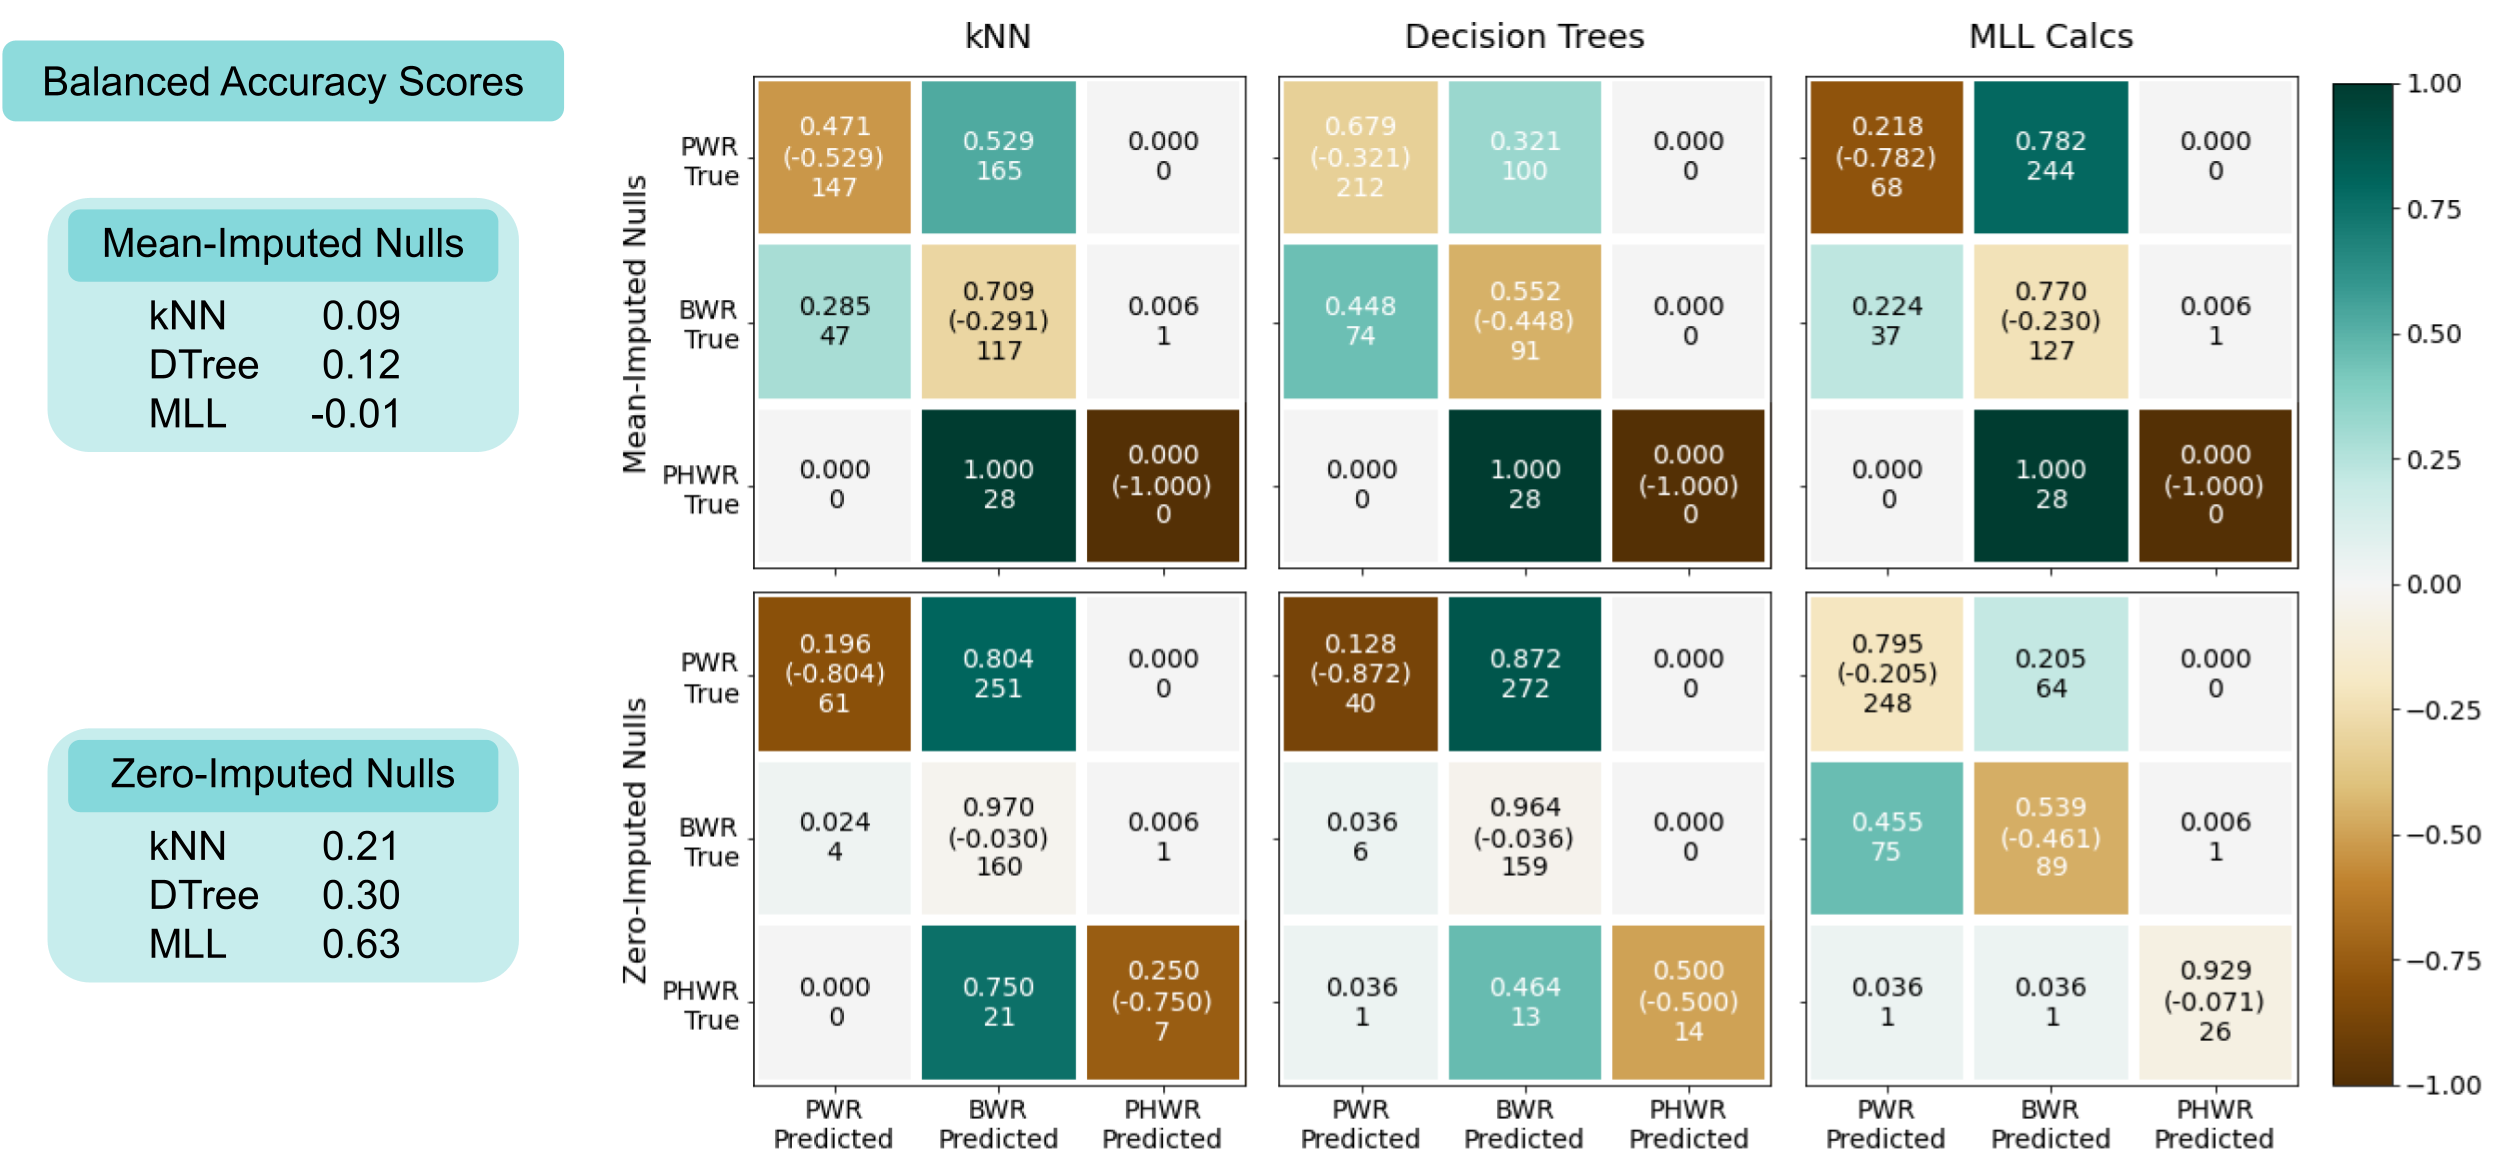
\includegraphics[height=0.68\textheight]{./figures/confusion_matrix_sfco.png}
  \end{figure}
\end{frame}

\begin{frame}
  \frametitle{SFCOMPO Prediction Results: Burnup}
  \vspace{-5pt}
  \begin{block}{Mean-Imputed Null Values}
    \begin{figure}
      \centering
      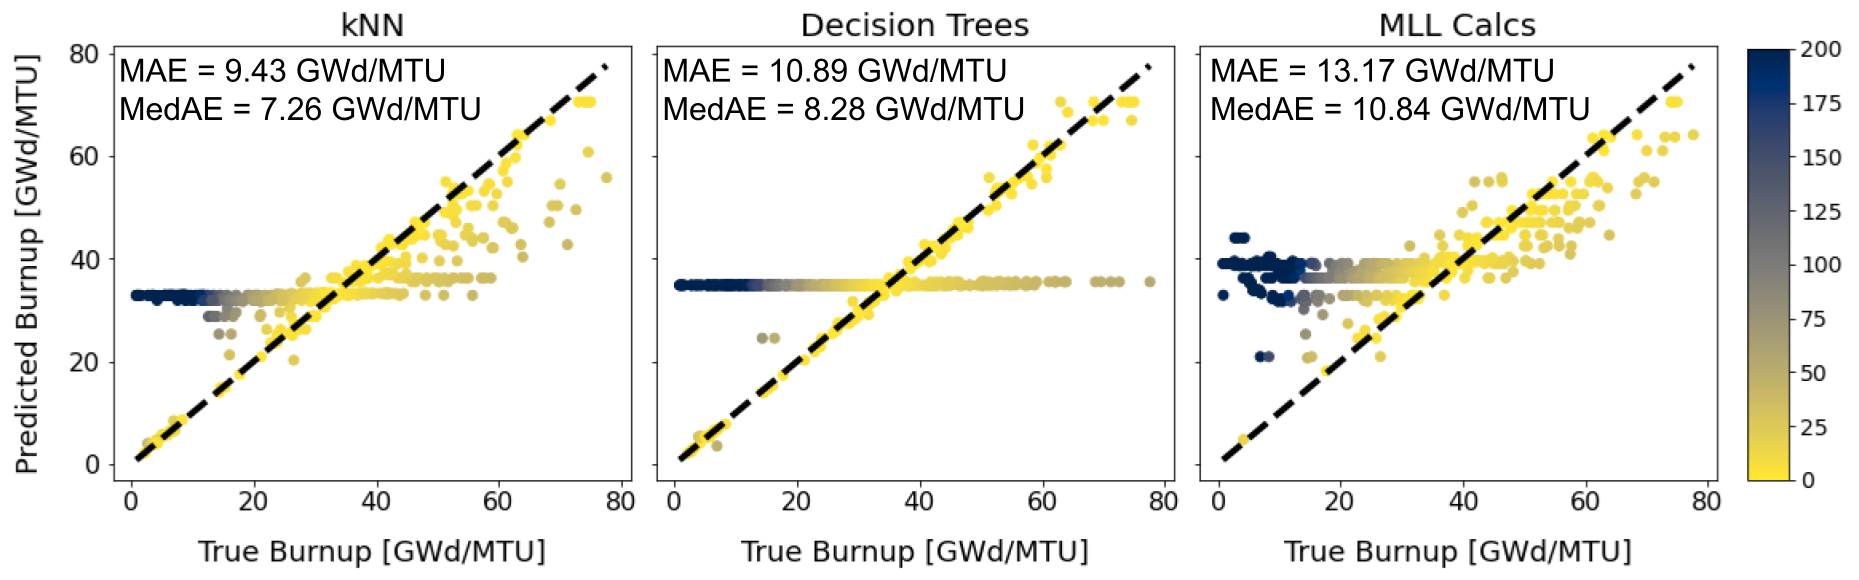
\includegraphics[height=0.35\textheight]{./figures/sfcompo_truey_vs_predy_impnull__burn.png}
    \end{figure}
  \end{block}
  \vspace{-5pt}
  \begin{block}{Zero-Imputed Null Values}
    \begin{figure}
      \centering
      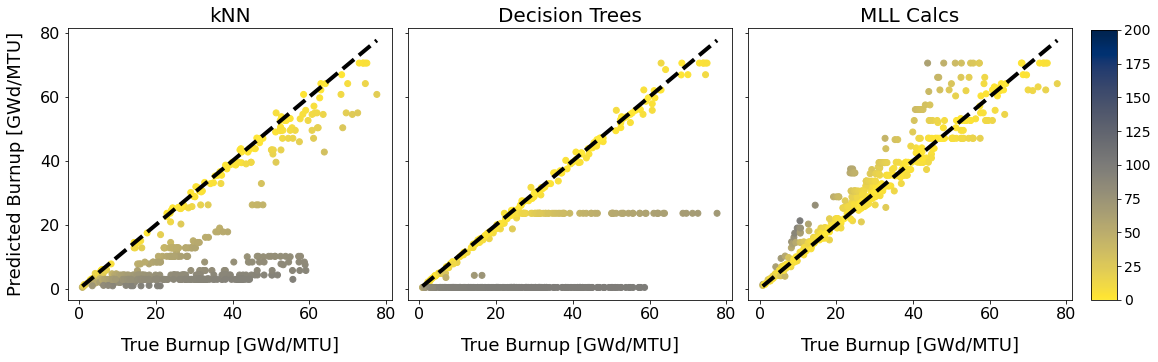
\includegraphics[height=0.35\textheight]{./figures/sfcompo_truey_vs_predy_0null__burn.png}
    \end{figure}
  \end{block}
\end{frame}

\begin{frame}
  \frametitle{SFCOMPO Prediction Results: ${}^{235}\text{U}$ Enrichment}
  \vspace{-5pt}
  \begin{block}{Mean-Imputed Null Values}
    \begin{figure}
      \centering
      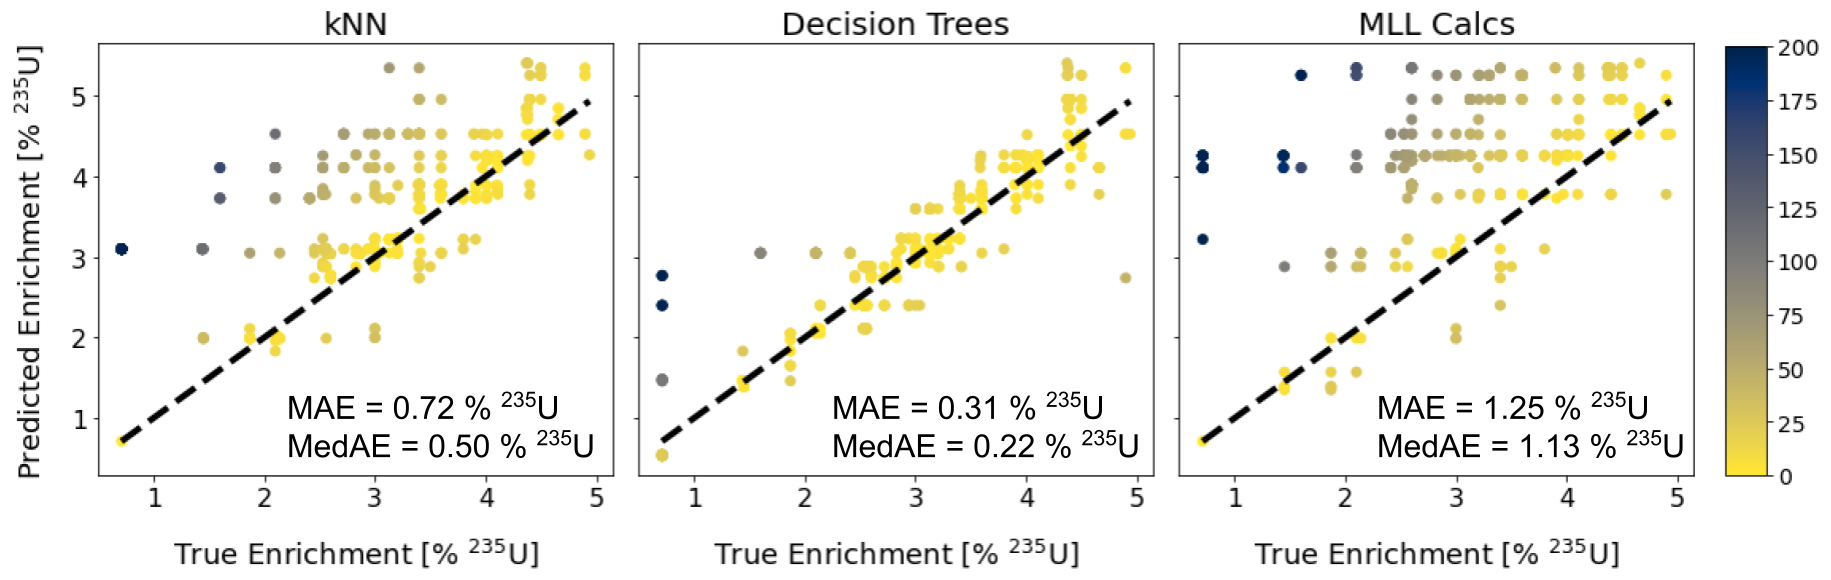
\includegraphics[height=0.35\textheight]{./figures/sfcompo_truey_vs_predy_impnull__enri.png}
    \end{figure}
  \end{block}
  \vspace{-5pt}
  \begin{block}{Zero-Imputed Null Values}
    \begin{figure}
      \centering
      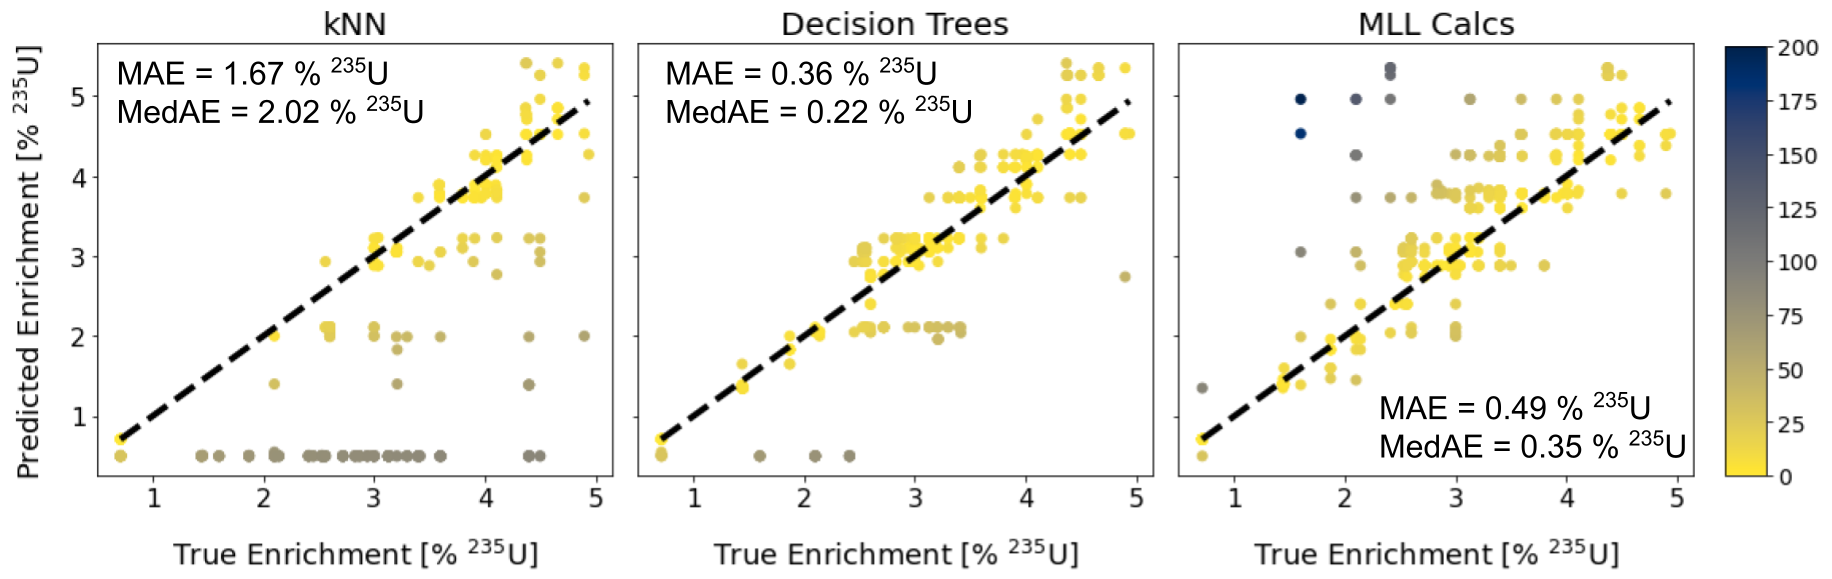
\includegraphics[height=0.35\textheight]{./figures/sfcompo_truey_vs_predy_0null__enri.png}
    \end{figure}
  \end{block}
\end{frame}

\begin{frame}
  \frametitle{Experiment Summary}
  \begin{itemize}
  \item Predictions with Nuclide Mass Random Error
    \begin{itemize}
      \item Impossible to determine boundary of acceptable/unacceptable
      \item Prediction performances at 20\% training set error are used as a
      minimum baseline for future work 
    \end{itemize}
  \item SFCOMPO
    \begin{itemize}
      \item Zero-imputed nulls performed better than mean-imputed nulls
      \item Challenges to using SFCOMPO with this methodology
    \end{itemize}
  \end{itemize}
\end{frame}

